\documentclass[../notes.tex]{subfiles}

\pagestyle{main}
\renewcommand{\chaptermark}[1]{\markboth{\chaptername\ \thechapter\ (#1)}{}}

\begin{document}




\chapter{Thinking Spectroscopically}
\section{Experimental Physical Chemistry: An Introduction}
\begin{itemize}
    \item \marginnote{1/3:}Questions:
    \begin{itemize}
        \item Is "Introduction to Nanotechnology by Linsay" the same as "Introduction to Nanoscience by Stuart M. Lindsay?"
        \begin{itemize}
            \item They'll check on this.
        \end{itemize}
        \item Access to Panopto recordings?
        \begin{itemize}
            \item I have access now.
        \end{itemize}
        \item Recordings of class content?
        \begin{itemize}
            \item Yes, if they can get the AV working.
        \end{itemize}
    \end{itemize}
    \item Intro by Hannah Lant (instructional professor to manage lab meetings). Tokmakoff handles lectures/non-in-lab stuff.
    \item Goals of the course.
    \begin{itemize}
        \item Demonstrate and interrogate principles from your theory courses, e.g., from QMech/Thermo.
        \item Learn practical techniques to characterize chemical and physical properties of molecules and nanomaterials, and the related spectroscopic techniques.
        \item Analysis of data (in-class and in-lab).
        \item What have you learned, and how can you communicate your findings to a scientific audience.
    \end{itemize}
    \item Everything helps everything else; it's cyclical from experimental theory, to collecting data, to data analysis, to communication, and back to more theory.
    \item Lectures will be more like workshops/recitations. There are recordings for content.
    \item Rest of today: Logistics and individual experiments.
    \item Canvas page.
    \begin{itemize}
        \item Syllabus.
        \item Most info on the Modules page.
        \item Fitting exercises will be in in-class meetings in the day to come.
        \item Experiments.
        \item Video lectures on Panopto.
    \end{itemize}
    \item Watch the 15-min Lecture 1 before class on Thursday!
    \item 6/9 weeks in lab. Complete a total of 6 experiments.
    \begin{itemize}
        \item Core experiments for weeks 2, 4-6 (UV/Vis, FT-IR, NMR, GC-MS).
        \begin{itemize}
            \item Full lab report on one of these; short lab report on the other ones.
        \end{itemize}
        \item Choose your experiments for weeks 7-8.
        \begin{itemize}
            \item Highlight content in nanomaterials and kinetics.
            \item Week 7 requires a full lab report on that experiment.
            \item Week 8 requires a group presentation on your experiment.
            \item Survey to determine what you do before Friday of Week 2!
        \end{itemize}
    \end{itemize}
    \item Grading breakdown.
    \begin{itemize}
        \item Prelab quizzes: 15\% (2.5\% per quiz).
        \begin{itemize}
            \item About 5 questions.
            \item Must get 80\% or above to attend lab.
            \item 2 attempts.
            \item Focus on safety, but also thinking critically about the theory for the lab.
        \end{itemize}
        \item Short reports: 40\% (10\% per report).
        \begin{itemize}
            \item How to do info --- in the lab manual.
            \item ACS citation style.
            \item There will be rubrics posted on Canvas (grading is not subject to the whims of our TAs).
        \end{itemize}
        \item Full reports: 30\% (15\% per report).
        \item Group oral presentation: 15\%.
        \begin{itemize}
            \item Attend a few other presentations and give ours during finals week.
        \end{itemize}
    \end{itemize}
    \item A full schedule of assignments and labs is available in the syllabus.
    \item See announcement for which lab cohort I'm supposed to be in!
    \item What the experiments are and what their purposes are (nontechnical because we haven't done the theory yet).
    \item Weeks 2, 4-6.
    \begin{itemize}
        \item UV/Vis to get a vibronic spectrum of iodine (to get electronic/vibrational data on \ce{I2}).
        \item FT-IR: Rovibrational information on \ce{HCl}.
        \item NMR: \ce{C5H11OH}.
        \item GC-MS: Separation science and MS. Analyze gasoline, which is a complex mixture of organic molecules.
    \end{itemize}
    \item Week 7 (+ info on who should choose these; think about it next week after first lab).
    \begin{itemize}
        \item Fluor: Fluorescence spectra of analytes, including pyrene.
        \begin{itemize}
            \item Both spectroscopy and kinetics. If you're really interested in physical chemistry and kinetics, do this. Uses custom built stuff in the labs.
        \end{itemize}
        \item QDots: Cadmium and Selenium nanocrystals.
        \begin{itemize}
            \item Applications of particle-in-a-box ideas, nanotechnology, synthesis, the prettiest one.
        \end{itemize}
        \item EChem: Developed by Anna Wuttig.
        \begin{itemize}
            \item More training in CV. Look at a number of different electrodes, and assay their activity in the hydrogen-evolution reaction. Applications in renewable energy.
            \item Will run both weeks 7-8.
            \item Includes some interaction with Wuttig.
        \end{itemize}
        \item AFM: Atomic force microscopy.
        \begin{itemize}
            \item Imaging a number of different materials, e.g., the grooves on a DVD. Great for anyone interested in nanoscience.
        \end{itemize}
    \end{itemize}
    \item Week 8:
    \begin{itemize}
        \item Photo: Alternate addition this week.
        \begin{itemize}
            \item Photodissociation of \ce{CO} from that hemoglobin structure and then some kinetics.
        \end{itemize}
    \end{itemize}
    \item The PChem lab suite: Enter Jones laboratory and turn left. We'll go elsewhere for special instrumentation. Lant's office is next door.
    \item NMR and GC-MS in Searle 340 instrumentation center. Usually meet our TA in the PChem lab suite and then travel.
    \item Attendance.
    \begin{itemize}
        \item You are required to attend all six lab sessions and record your own data (often in groups).
        \item Excused absences include university travel, family emergencies, and illness; please be in touch with Prof. Lant as soon as possible to reschedule your lab.
        \item Unexcused absences may be able to reschedule at a 20\% penalty if availability allows (this is an overenrolled class).
    \end{itemize}
    \item Safety.
    \begin{itemize}
        \item General lab safety policies from Gen Chem and OChem still apply.
        \item Bring your own goggles.
        \item Acknowledge you've reviewed the polices on Canvas in the first lab quiz.
        \item Safety tour of the lab space on your first lab day by your TA.
        \item Lab aprons will be provided.
        \item Specific safety concerns will be communicated in lab manuals and pre-lab quizzes.
    \end{itemize}
    \item We're all coming in with diverse scientific experiences. Fill out a survey on Canvas $>$ Assignments $>$ surveys or at \href{https://www.tinyurl.com/pchemlabsurvey}{tinyurl.com/pchemlabsurvey}!
    \item No formal lecture on Thursday in this room! There will be a series of about 7 video lectures over the first two weeks that cover what we need to know for our first core experiments (watch these!). Workshops during this period, too. E.g., if they find from the surveys that we don't have experience with fitting data very well, we'll work through that. There is an exercise for this on Canvas?? (Data Fitting Exercises.pdf explains it.)
    \item Tokmakoff puts a big emphasis on communication :)
    \begin{itemize}
        \item "Any professional science is communicated; otherwise, it's just a hobby."
        \item Should be nicely formatted with good figures, etc.
    \end{itemize}
    \item My lab group: Thursday A.
    \item Schedule.
    \begin{itemize}
        \item UV/Vis: 1/12.
        \item FT-IR: 1/26.
        \item NMR: 2/2.
        \item GC-MS: 2/9.
    \end{itemize}
\end{itemize}



\section{Lecture 1: Principles of Spectroscopy}
\begin{itemize}
    \item \textbf{Spectroscopy}: Studying the properties of matter (e.g., molecules and materials) through its interaction with different frequency components of the electromagnetic spectrum. \emph{Etymology} \textbf{spectron} from Latin "ghost" or "spirit."
    \begin{itemize}
        \item More on the etymology: An apt description because you never see the molecule itself; you see a representation/image/apparition of it.
    \end{itemize}
    \item Each type of spectroscopy gives a different picture (the \emph{spectrum}).
    \begin{figure}[h!]
        \centering
        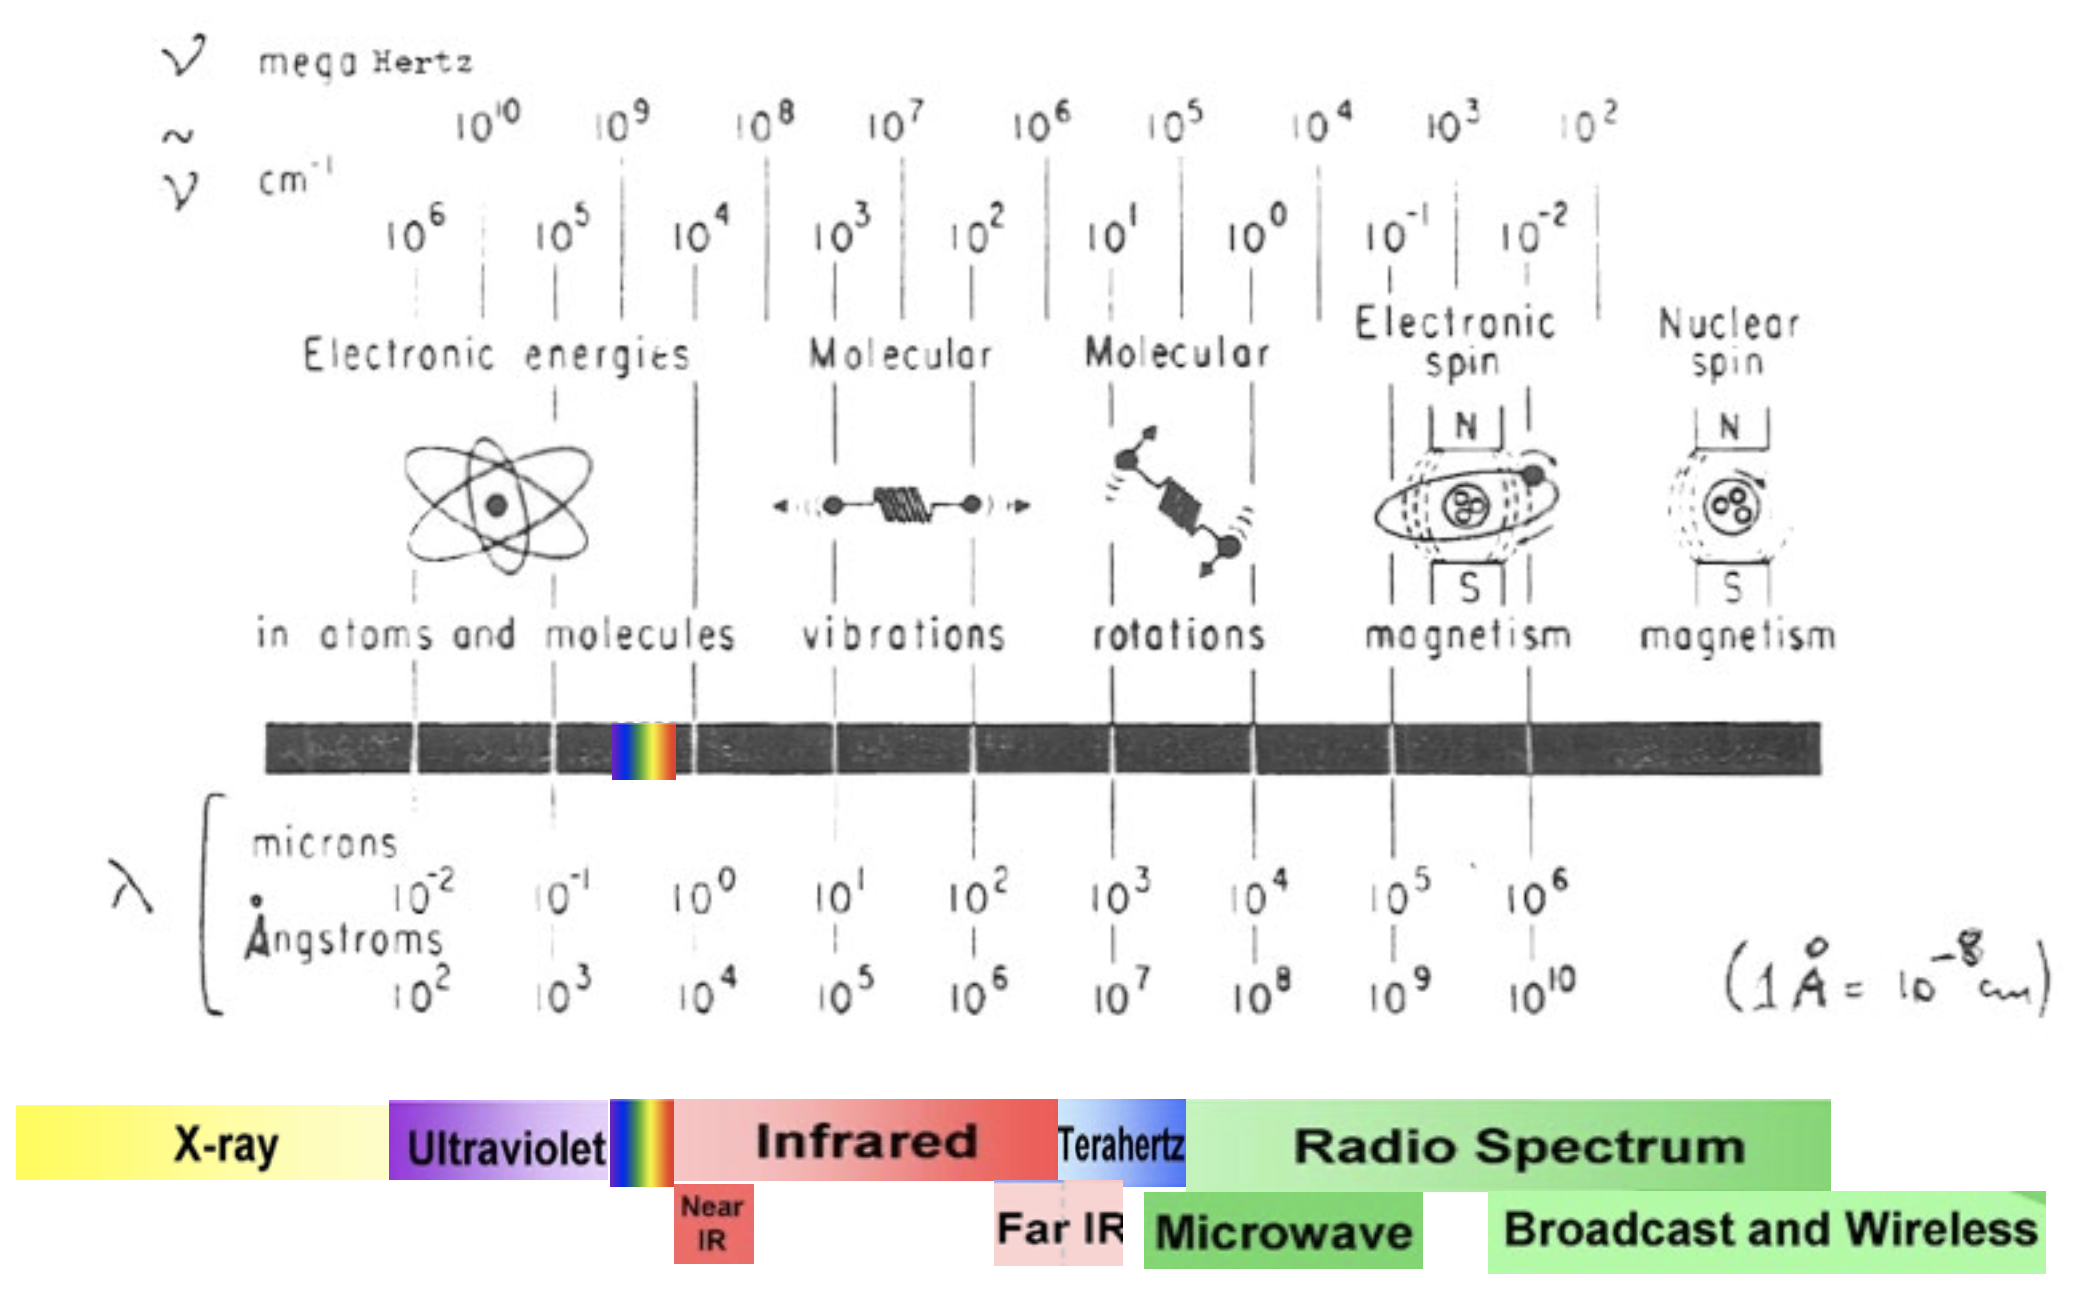
\includegraphics[width=0.68\linewidth]{spectroscopicSpectrum.png}
        \caption{Types of light used by different forms of spectroscopy.}
        \label{fig:spectroscopicSpectrum}
    \end{figure}
    \begin{itemize}
        \item UV/Vis: Electronic absorption (esp. valence electrons).
        \item Infrared: Vibrations.
        \item Microwave: Rotations and crystal lattice vibration.
        \item Radio: NMR.
    \end{itemize}
    \item Goals.
    \begin{itemize}
        \item Understand how light interacts with matter and how you can use this to quantitatively understand your sample (e.g., molecular structure, dynamics, reactivity).
        \item Understand spectroscopy the way you understand other common tools of measurement (like a ruler).
        \item See that spectroscopy is a set of tools that you can put together in different ways to solve the chemical problems that are of interest to you.
    \end{itemize}
    \item A spectrum measures\dots
    \begin{itemize}
        \item The interaction of light with a sample influences the sample and the light.
        \item Two universal steps: Excitation and detection.
        \item Light passes through the sample and then gets characterized on its way out (e.g., absorption, emission, scattering, reflection, dispersion, rotation). We can also characterize a change in the sample (e.g., photothermal, photoelectron and ionization, photochemistry).
        \item In most cases, we characterize how a sample modifies the incident light.
    \end{itemize}
    \item Two common measurements.
    \item \textbf{Absorption}: The attenuation of a light field passing through a sample.
    \begin{itemize}
        \item Photodetectors measure intensity, which is related to the square of the electric field.
    \end{itemize}
    \item \textbf{Emission}: Excitation induces light emission from the sample, typically of a different frequency.
    \item \textbf{Fluorescence}: Emission from singlet states.
    \item \textbf{Phosphoresence}: Emission from triplet states.
    \item \textbf{Raman scattering}: Light taken up shifts the frequency.
    \item The basics of an absorption spectrum.
    \begin{figure}[h!]
        \centering
        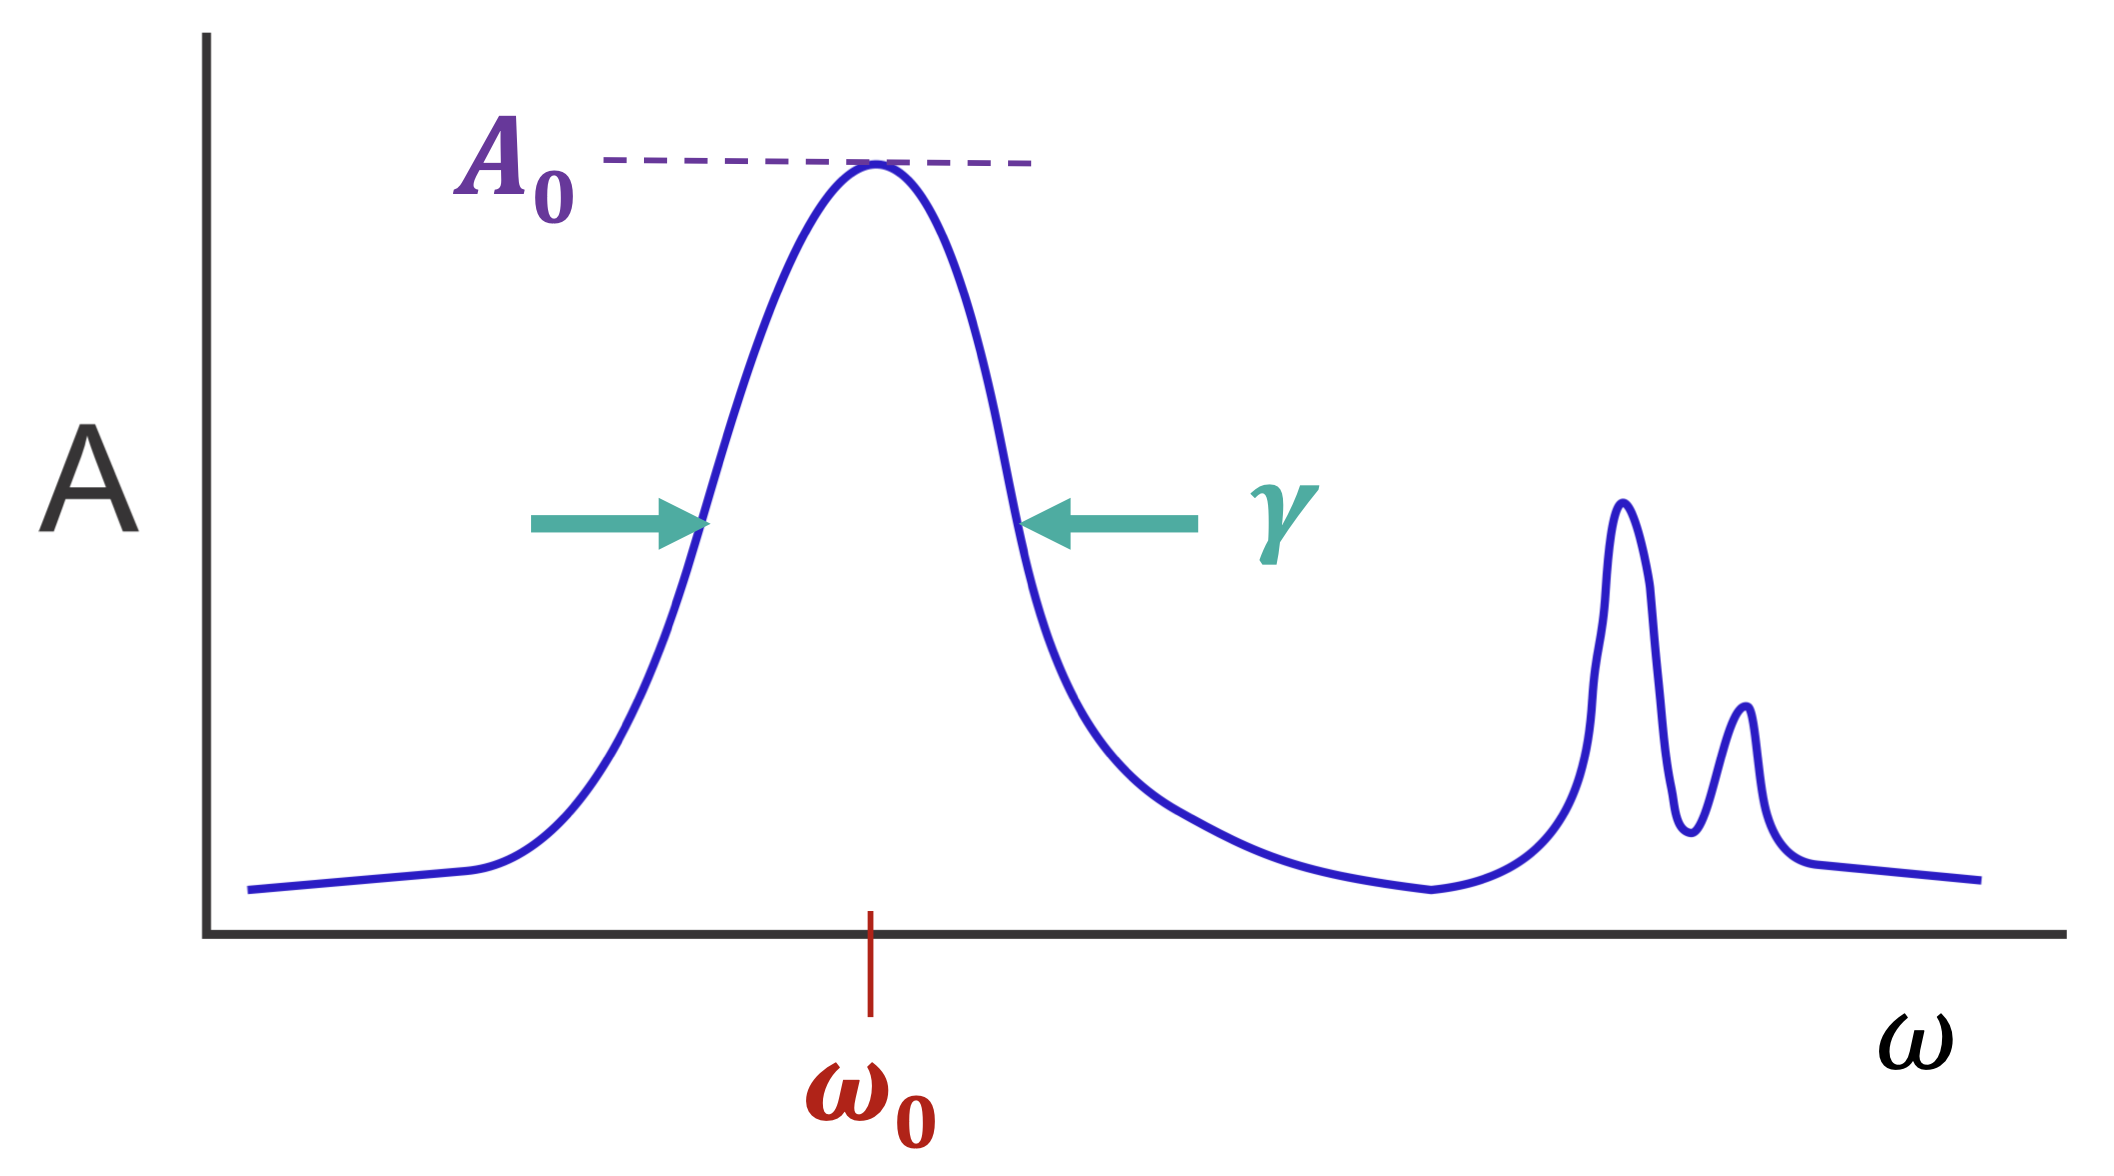
\includegraphics[width=0.35\linewidth]{spectrumFeatures.png}
        \caption{Features of an absorption spectrum.}
        \label{fig:spectrumFeatures}
    \end{figure}
    \begin{itemize}
        \item $x$-axis: Characterizes the input light in terms of frequency (frequency, angular frequency, or wavenumber), wavelength, or energy.
        \item $y$-axis: How the intensity of the light was attenuated at a particular frequency. Look at transmission ($T=I/I_0$) or absorbance ($A=-\log T=\epsilon(\nu)CL$, where $\epsilon$ is the extinction coefficient [unit \si{\liter\per\mole\per\centi\meter}], $C$ is the concentration [unit \si{\molar}], and $L$ is the sample pathlength [unit \si{\centi\meter}]).
        \item Features: Resonance frequency $\omega_0$, peak height $A_0$ or peak area, linewidth $\gamma$ (different frequencies absorbed; gives information on dynamical processes), lineshape (actual functional form of the peak).
    \end{itemize}
    \item How do you measure absorption spectra?
    \begin{itemize}
        \item Measure the change of intensity of light at different frequencies as it passes through a sample.
        \item Two types of spectrometers: Dispersive (common for visible spectrometers) and Fourier transform (more on this later).
    \end{itemize}
    \item \textbf{Dispersive spectrometer}: A spectrometer that has a dispersive element, that is, one that takes white light and spacially spreads the colors of the rainbow.
    \begin{itemize}
        \item Could be a reflection grating, prism, etc.
        \item Measure the white light without the sample, and then with the sample and see what changes. Calculate the transmission, and then absorbance.
    \end{itemize}
    \item That was basic definitions and variables.
    \item This time: We have defined some basic variables for an absorption spectrum.
    \item Next time: Molecular interactions of light. Analyze this mode: Driven electron on a spring.
\end{itemize}



\section{Lecture 2: A Classical Model for Absorption Spectroscopy}
\begin{itemize}
    \item \marginnote{1/5:}Last time: Absorption spectra features.
    \item Today: Building intuition about how molecules absorb light and what we can learn about them from this.
    \item Picture absorption of light from a quantum mechanical perspective.
    \begin{itemize}
        \item Photons with energy that match the energy difference between certain energy levels excite electrons.
        \item This is true, but it doesn't tell us much about the molecule itself. Thus, let's gain insight from a classical model of absorption.
    \end{itemize}
    \item Why is there light absorption?
    \begin{itemize}
        \item Classically, light interacts with \emph{charges}.
        \begin{itemize}
            \item Molecules are composed of charged particles (e.g., electrons and protons).
            \item An electromagnetic field $E$ exerts a force $F$ on these charges $q$ via
            \begin{equation*}
                F = qE
            \end{equation*}
        \end{itemize}
        \item A classical model of absorption: Start with $F=ma$.
        \begin{itemize}
            \item How do we describe light? As an oscillating electromagnetic field.
            \item How do we describe matter? As a harmonic oscillator.
            \item How do we describe the interaction? An oscillating EM field drives the harmonic oscillator.
        \end{itemize}
    \end{itemize}
    \item Review of electromagnetic radiation.
    \begin{itemize}
        \item EM radiation: A traveling wave in the EM field that oscillates in time and space orthogonal to the direction of motion in both of the (orthogonal) $E$ and $B$ fields.
        \item These waves have a characteristic periodicity $\lambda$ called the \textbf{wavelength} that is inversely proportional to the \textbf{wavevector} $k$ via
        \begin{equation*}
            \lambda = \frac{2\pi}{k}
        \end{equation*}
        \item The electric field vector $\hat{\varepsilon}$ --- also known as the polarization of the light field --- is orthogonal to the direction of propagation.
        \item Since speed is fixed, the spacial periodicity is linked to time. Hence, the period $\tau=2\pi/\omega=1/\nu$.
        \item Important equation: The variables in this equation are the most important ones we'll deal with in one form or another during this class.
        \begin{equation*}
            \bar{E}(\bar{r},t) = \hat{\varepsilon}E_0\cos(\omega t-\bar{k}\cdot\bar{r})
        \end{equation*}
        \begin{itemize}
            \item $\bar{\varepsilon}$ is the polarization vector.
            \item The electric field amplitude $E_0$ is our main observable, and we primarily deal with it through the intensity $I=\frac{1}{2}\varepsilon_0|E_0|^2$.
            \item $\omega$ is the frequency in radians per second. In class, we'll typically use $\nu=\omega/2\pi$, though.
            \item $\bar{k}$ is the wavevector.
        \end{itemize}
        \item For our model, we'll drop several of the variables to yield
        \begin{equation*}
            E(t) = E_0\cos(\omega t)
        \end{equation*}
        \begin{itemize}
            \item We drop all vector quantities (i.e., $\hat{\varepsilon},\bar{k}$) to simplify the math.
            \item We can drop the wavevector because all of the particles that the light will interact with are spacially localized in a much smaller area than the wavelength. Thus, the spatial variation of the field can be neglected.
        \end{itemize}
    \end{itemize}
    \item \textbf{Wavevector}: A vector that defines the direction in which the light travels at the speed of light. \emph{Denoted by} $\bm{k}$.
    \item Molecules consist of bound charges.
    \begin{itemize}
        \item Why is it reasonable to treat a charged particle in a molecule as a harmonic oscillator? Because electrons and nuclei in molecules have well defined equilibria and thus feel a restoring force when a field pushes them away from equilibrium.
        \item Example: For nuclei, bond length is a balance between attractive and repulsive forces (think Lennard-Jones potential).
        \item Example: For electrons, orbitals represent a distribution that can be distorted.
        \item Example: For nuclear and electronic spins, a magnetic field aligns spins with the field and a secondary radio-frequency field tries to flip them.
    \end{itemize}
    \item Relating bound charge variables to harmonic oscillator variables.
    \begin{itemize}
        \item We approximate the very bottom of the Lennard-Jones potential well as a parabola. This is justified by the Taylor series expansion of the potential at the minimum.
        \item The curvature at the bottom is the force constant in a harmonic potential.
        \begin{equation*}
            F_\text{res} = -\pdv{V}{x} = -kQ
        \end{equation*}
        \item Note that $Q$ is the displacement from equilibrium.
    \end{itemize}
    \item Assembling the classical model.
    \begin{itemize}
        \item Derive an equation of motion for the charged particle of mass $m$: Use $F=ma$.
        \item Inputs:
        \begin{itemize}
            \item Light: $E(t)=E_0\cos(\omega t)$.
            \item Matter: $F_\text{res}=-kQ$.
            \item Interaction: $F_\text{ext}=qE(t)=qE_0\cos(\omega t)$.
        \end{itemize}
        \item Expanding Newton's second law with the inputs, we obtain
        \begin{align*}
            m\pdv[2]{Q}{t} = F_\text{res}+F_\text{ext}
        \end{align*}
    \end{itemize}
    \item To rationalize the final harmonic oscillator result, let's slowly add in different contributions to the force instead of starting all at once.
    \begin{itemize}
        \item We'll do this in three steps: No external force, damping, and damping plus external driving force.
    \end{itemize}
    \item Harmonic oscillator with no external force.
    \begin{itemize}
        \item The equation of motion is
        \begin{equation*}
            m\pdv[2]{Q}{t}+kQ = 0
        \end{equation*}
        \item The solution is
        \begin{equation*}
            Q(t) = A\sin(\omega_0t)+B\cos(\omega_0t)
        \end{equation*}
        where $\omega_0=\sqrt{k/m}$ is the \textbf{harmonic frequency} of the oscillator.
        \item The exact nature of the solution will depend on initial conditions.
        \begin{itemize}
            \item If we hold the particle away from equilibrium and release it at $t=0$, we'll need cosine.
            \item If we kick it away from equilibrium at $t=0$, we'll need sine.
        \end{itemize}
        \item For now, we'll consider only the sine solutions (i.e., take $B=0$).
    \end{itemize}
    \item Harmonic oscillator with damping.
    \begin{itemize}
        \item The equation of motion is
        \begin{equation*}
            m\pdv[2]{Q}{t} = F_\text{res}+F_\text{damp} = -kQ-b\pdv{Q}{t}
        \end{equation*}
        \begin{itemize}
            \item This harmonic oscillator doesn't just oscillate periodically forever, but dissipates its energy at a characteristic rate $b$.
        \end{itemize}
        \item Two reasons to include damping.
        \begin{itemize}
            \item It simplifies the math a bit.
            \item It tells us how irreversible relaxation processes influence spectra (we'll measure this in our NMR experiment). Think about it as a correction for physical reality: No harmonic oscillator is a perpetual motion machine, i.e., they all lose energy to friction, heat, or something else.
        \end{itemize}
        \item The solution is
        \begin{equation*}
            Q(t) = A\e[-\gamma t]\sin(\Omega_0t)
        \end{equation*}
        with \textbf{reduced frequency} and \textbf{damping constant}
        \begin{align*}
            \Omega_0 &= \sqrt{\omega_0^2-\gamma^2}&
            \gamma &= \frac{b}{2m}
        \end{align*}
        respectively.
        \item In our scenario, we'll imagine that damping is weak, i.e., that $\omega_0\gg\gamma$ so that $\Omega_0\approx\omega_0$.
    \end{itemize}
    \item Harmonic oscillator with the external driving force.
    \begin{itemize}
        \item The equation of motion is
        \begin{align*}
            m\pdv[2]{Q}{t} &= F_\text{res}+F_\text{damp}+F_\text{ext}\\
            &= -kQ-b\pdv{Q}{t}+F_\text{ext}\\
            \pdv[2]{Q}{t}+2\gamma\pdv{Q}{t}+\omega_0^2Q &= \frac{F_0}{m}\cos\omega t
        \end{align*}
        \begin{itemize}
            \item Note that we have defined $F_0=qE_0$ to be the maximum force that the field exerts on the oscillator, where we recall that $E_0$ is the maximum magnitude (amplitude) of the electromagnetic field.
        \end{itemize}
        \item Solution: We get a driven particle that oscillates as a sine but with a different phase. Mathematically,
        \begin{equation*}
            Q(t) = A\sin(\omega t+\beta)
        \end{equation*}
        where
        \begin{align*}
            A &= \frac{F_0}{2m\omega_0}\frac{1}{\sqrt{(\omega_0-\omega)^2+\gamma^2}}&
            \tan\beta &= \frac{\omega_0^2-\omega^2}{2\gamma\omega}
        \end{align*}
        \item Observations:
        \begin{itemize}
            \item When we're \textbf{on resonance}, we get the largest displacement of the particle by the field. This is the most efficient point at which we can drive the charged particle to move. This is evident from the denominator of $A$ (i.e., $A$ is maximized when $\omega_0-\omega=0$).
            \item The particle oscillates at the driving frequency $\omega$, not $\omega_0$.
            \item The particle oscillates \ang{90} out of phase with the external force field when on resonance.
        \end{itemize}
    \end{itemize}
    \item \textbf{On resonance} (oscillation): An oscillation for which the driving frequency of the external field matches the natural resonance frequency of the harmonic oscillator, i.e., $\omega\approx\omega_0$.
    \item Now we can actually go and calculate an absorption spectrum.
    \begin{figure}[H]
        \centering
        \begin{tikzpicture}[scale=0.8]
            \footnotesize
            \draw [-stealth] (-3.2,0) -- (3.2,0) node[right]{$\omega$};
            \draw (0,0.1) -- ++(0,-0.2) node[below]{$\omega^{}_0$};
    
            \draw [rex,thick] plot[domain=-3:3,samples=500,smooth] (\x,{1/(3*(\x*\x+1/9))});
    
            \draw [<-,shorten <=2pt] ({1/3},1.5) -- ++(0.4,0) node[right]{$2\gamma$};
            \draw [<-,shorten <=2pt] ({-1/3},1.5) -- ++(-0.4,0);
            \draw [dashed] (-0.2,3.03) -- ++(0.7,0) node[right]{$\displaystyle\frac{F_0^2}{2m\gamma}$};
    
            \node at (-2,0.5) {\small$P_\text{avg}(\omega)$};
        \end{tikzpicture}
        \caption{Lorentzian lineshape.}
        \label{fig:Lorentzian}
    \end{figure}
    \begin{itemize}
        \item We do this by calculating the power absorbed by the oscillator.
        \item We take $\text{power}=\text{force}\times\text{velocity}$ and, as a time-dependent quantity, average it over one cycle.
        \item Mathematically, we get
        \begin{equation*}
            P_\text{avg} = \left\langle F(t)\cdot\pdv{Q}{t} \right\rangle_\text{avg}
            = \frac{\gamma F_0^2}{2m}\frac{1}{(\omega-\omega_0)^2+\gamma^2}
        \end{equation*}
        \begin{itemize}
            \item Note that the resonance denominator implies that $P_\text{avg}$ is maximized when the particle is on resonance.
        \end{itemize}
        \item The curve $P_\text{avg}(\omega)$ is a \textbf{Lorentzian lineshape}.
        \begin{itemize}
            \item The peak is at the resonance frequency $\omega_0$.
            \item The width is twice the damping coefficient when we define the width to be the "full width of the line at half of the maximum height."
            \item The amplitude is related to the square of the maximum magnitude of the driving force, as well as corrections for the mass and the damping coefficient. Alternatively, the area under the curve is $\pi F_0^2/4m$.
        \end{itemize}
        \item Thus, we have related three important parameters in our model --- which is meant to represent molecules --- to the spectrum.
    \end{itemize}
    \item So how does this model help us study molecules quantitatively?
    \begin{itemize}
        \item First and foremost, the model provides a dynamic interpretation of spectroscopy.
        \item There are experimental observables such as the line width, resonance frequency, and amplitude that are directly related to molecular observables.
        \item Most of these results are directly applicable to molecules. These classical analogies work quite well in many cases. Some modifications are needed in more sophisticated cases, though. For example, for multiple particles and charges, we (1) replace the mass with the reduced mass and (2) integrate point charges into the dipole moment.
    \end{itemize}
    \item Example of the model helping us: Analysis of the IR spectrum of ethyl acetate.
    \begin{itemize}
        \item Suppose we want to learn a bit more about the \ce{C=O} bond.
        \item Observe that $\bar{\nu}\approx\SI{1750}{\per\centi\meter}$ and the line width is about \SI{30}{\per\centi\meter} for the \ce{C=O} absorption.
        \item Since $\bar{\nu}=\nu c=\omega_0/2\pi c$, the vibrational period of the \ce{C=O} bond is $\tau=1/\nu=2\pi/\omega_0\approx\SI{19}{\femto\second}$.
        \item $k$, the curvature of the \ce{C=O} potential, tells us the bond stiffness (which is closely related to bond strength and bond order) is $k=m_R\omega_0^2$.
        \item $\gamma$ tells us the energy dissipation time. Invert the line width (i.e., take $1/\gamma$) to get an effective time scale for the time to dissipate the energy you put into the bond (about \SI{2}{\pico\second}). Thus, if you kick the bond, it's going to oscillate many times (every \SI{19}{\femto\second}) before it dissipates half its energy (in \SI{2000}{\femto\second}).
    \end{itemize}
    \item In addition to analytical power, the model gives us predictive power.
    \begin{itemize}
        \item How can we be confident in our vibrational assignment? The model predicts an isotope effect, i.e., that the resonance frequency $\omega_0$ will scale inversely with the reduced mass $m_R$ via
        \begin{equation*}
            \omega_0 = \sqrt{\frac{k}{m_R}}
        \end{equation*}
        \item Example (comparing two molecules): If we know one molecule's resonance frequency, we can predict another via
        \begin{equation*}
            \frac{\bar{\nu}_1}{\bar{\nu}_2} = \sqrt{\frac{m_{R,2}}{m_{R,1}}}
        \end{equation*}
        \item Example: $m_R(\ce{H{}^35Cl})=0.97$ and $m_R=(\ce{D{}^35Cl})=1.89$, so if $\bar{\nu}$ for \ce{{}^1H{}^35Cl} is \SI{2890}{\per\centi\meter}, we predict that $\bar{\nu}$ for \ce{{}^2H{}^35Cl} is \SI{2070}{\per\centi\meter}, and indeed that is very close to the measured value.
    \end{itemize}
    \item What, molecularly, gives rise to $F_0$?
    \begin{itemize}
        \item Molecules are different than the case of a single bound charge because (1) they contain many bound charges (multiple protons and electrons) and (2) they are neutral overall.
        \item However, the distribution of these charges in space (the \textbf{dipole moment}) can be influenced and changed by the light field.
        \item Thus, we want to understand the forces that the electromagnetic field exerts on the dipole moment.
        \item The force exerted by the electric field on the dipole can be derived from the potential energy. We know from classical mechanics that the potential energy of a dipole in an electric field is $V=-\bar{\mu}\cdot\bar{E}$ and that $F=-\pdv*{V}{Q}$, so we must have
        \begin{equation*}
            F = -\pdv{V}{Q} = \left( \pdv{\bar{\mu}}{Q} \right)\cdot\bar{E}
        \end{equation*}
        \begin{itemize}
            \item The final expression implies that in order for the force exerted by the EM field on the molecule to be nonzero, the dipole moment must change with molecular coordinate being driven.
            \item Example: \ce{CO2} is such a strong absorber of IR radiation even though its nonpolar because it's \emph{bending} mode breaks the symmetry and allows its dipole to change.
        \end{itemize}
    \end{itemize}
    \item \textbf{Dipole moment}: The distribution of the charges in a molecule in space. \emph{Denoted by} $\bm{\mu},\bm{\bar{\mu}}$. \emph{Given by}
    \begin{equation*}
        \bar{\mu} = \sum_{i\text{ charges}}q_i\bar{r}_i
    \end{equation*}
    \begin{itemize}
        \item This is a vector quantity.
    \end{itemize}
    \item Light inducing a dipole change.
    \begin{figure}[H]
        \centering
        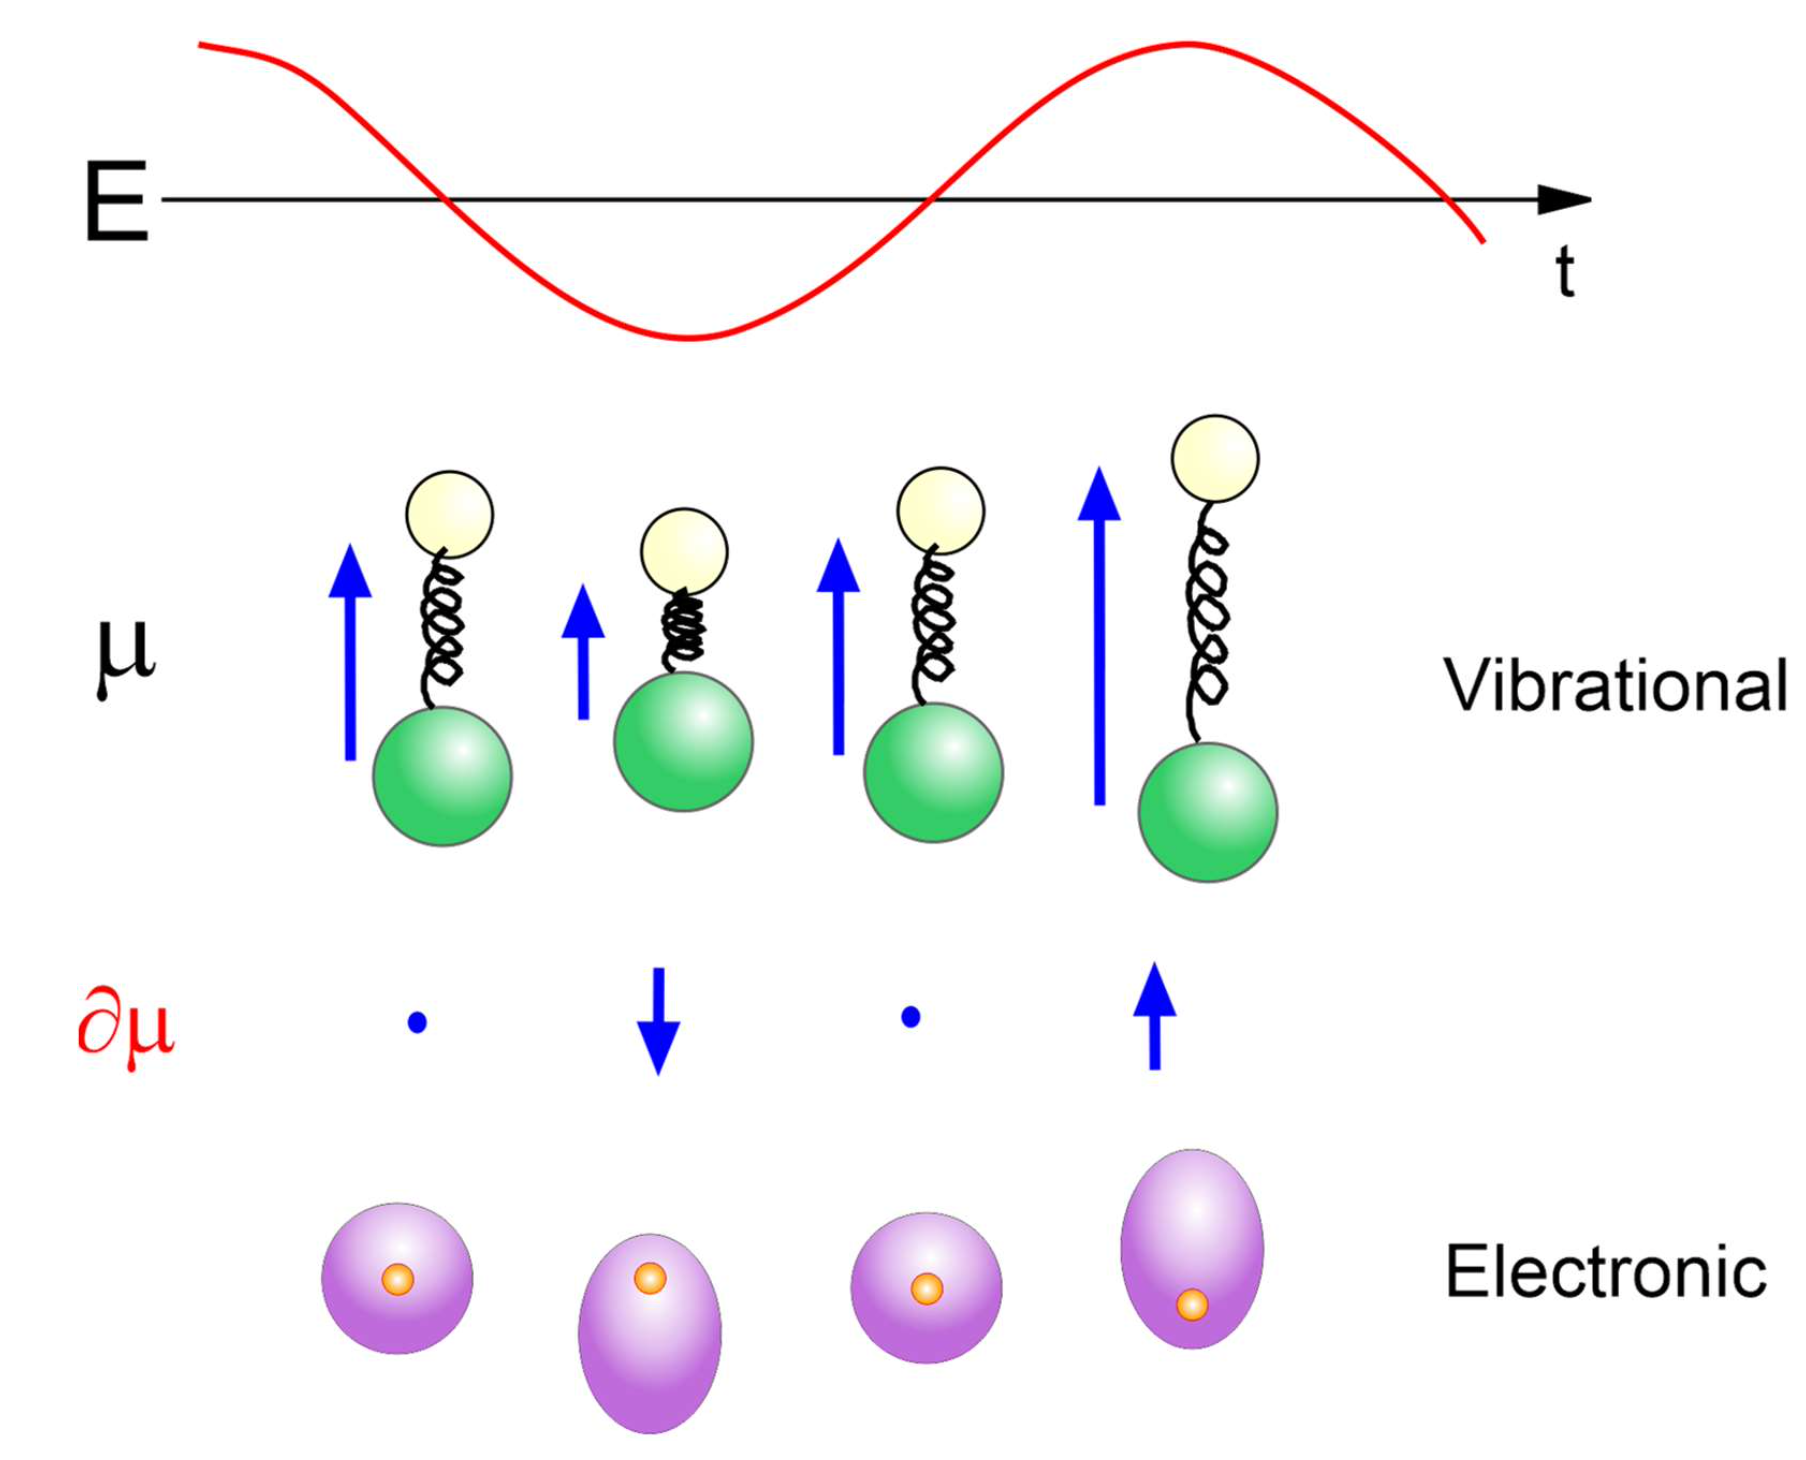
\includegraphics[width=0.4\linewidth]{EMdipoleChange.png}
        \caption{Light inducing a dipole change.}
        \label{fig:EMdipoleChange}
    \end{figure}
    \begin{itemize}
        \item The largest forces on the bond occur at the extrema of the field.
        \item A very similar thing happens in electronic spectroscopy. There, though, we don't have a \emph{bond} vibration but assume that the overall \emph{electron cloud} of an atom is polarizable and can oscillate.
    \end{itemize}
    \item The interaction depends on alignment.
    \begin{itemize}
        \item $E$ oscillates along the polarization vector $\hat{\varepsilon}$.
        \item The interaction depends on the alignment of the dipole $\bar{\mu}$ with $\hat{\varepsilon}$.
        \item The strongest interaction occurs when the dipole moments of the molecules are aligned with the polarization of the electric field, but if they're orthogonal, then they don't interact at all.
        \item Thus, we need a dot product, and we take
        \begin{align*}
            F_\text{ext}(t) &= \left| \pdv{\bar{\mu}}{Q} \right|\cdot\bar{E}(t)&
            F_0 &= \pdv{\mu}{Q}E_0\cos\theta
        \end{align*}
        \item In a sample of many molecules, we have to average over all of them.
        \item Used to investigate\dots
        \begin{itemize}
            \item The orientation of bonds in crystals;
            \item Rotational motion in liquids or gas.
        \end{itemize}
    \end{itemize}
    \item Absorption through rotation of a dipole.
    \begin{figure}[h!]
        \centering
        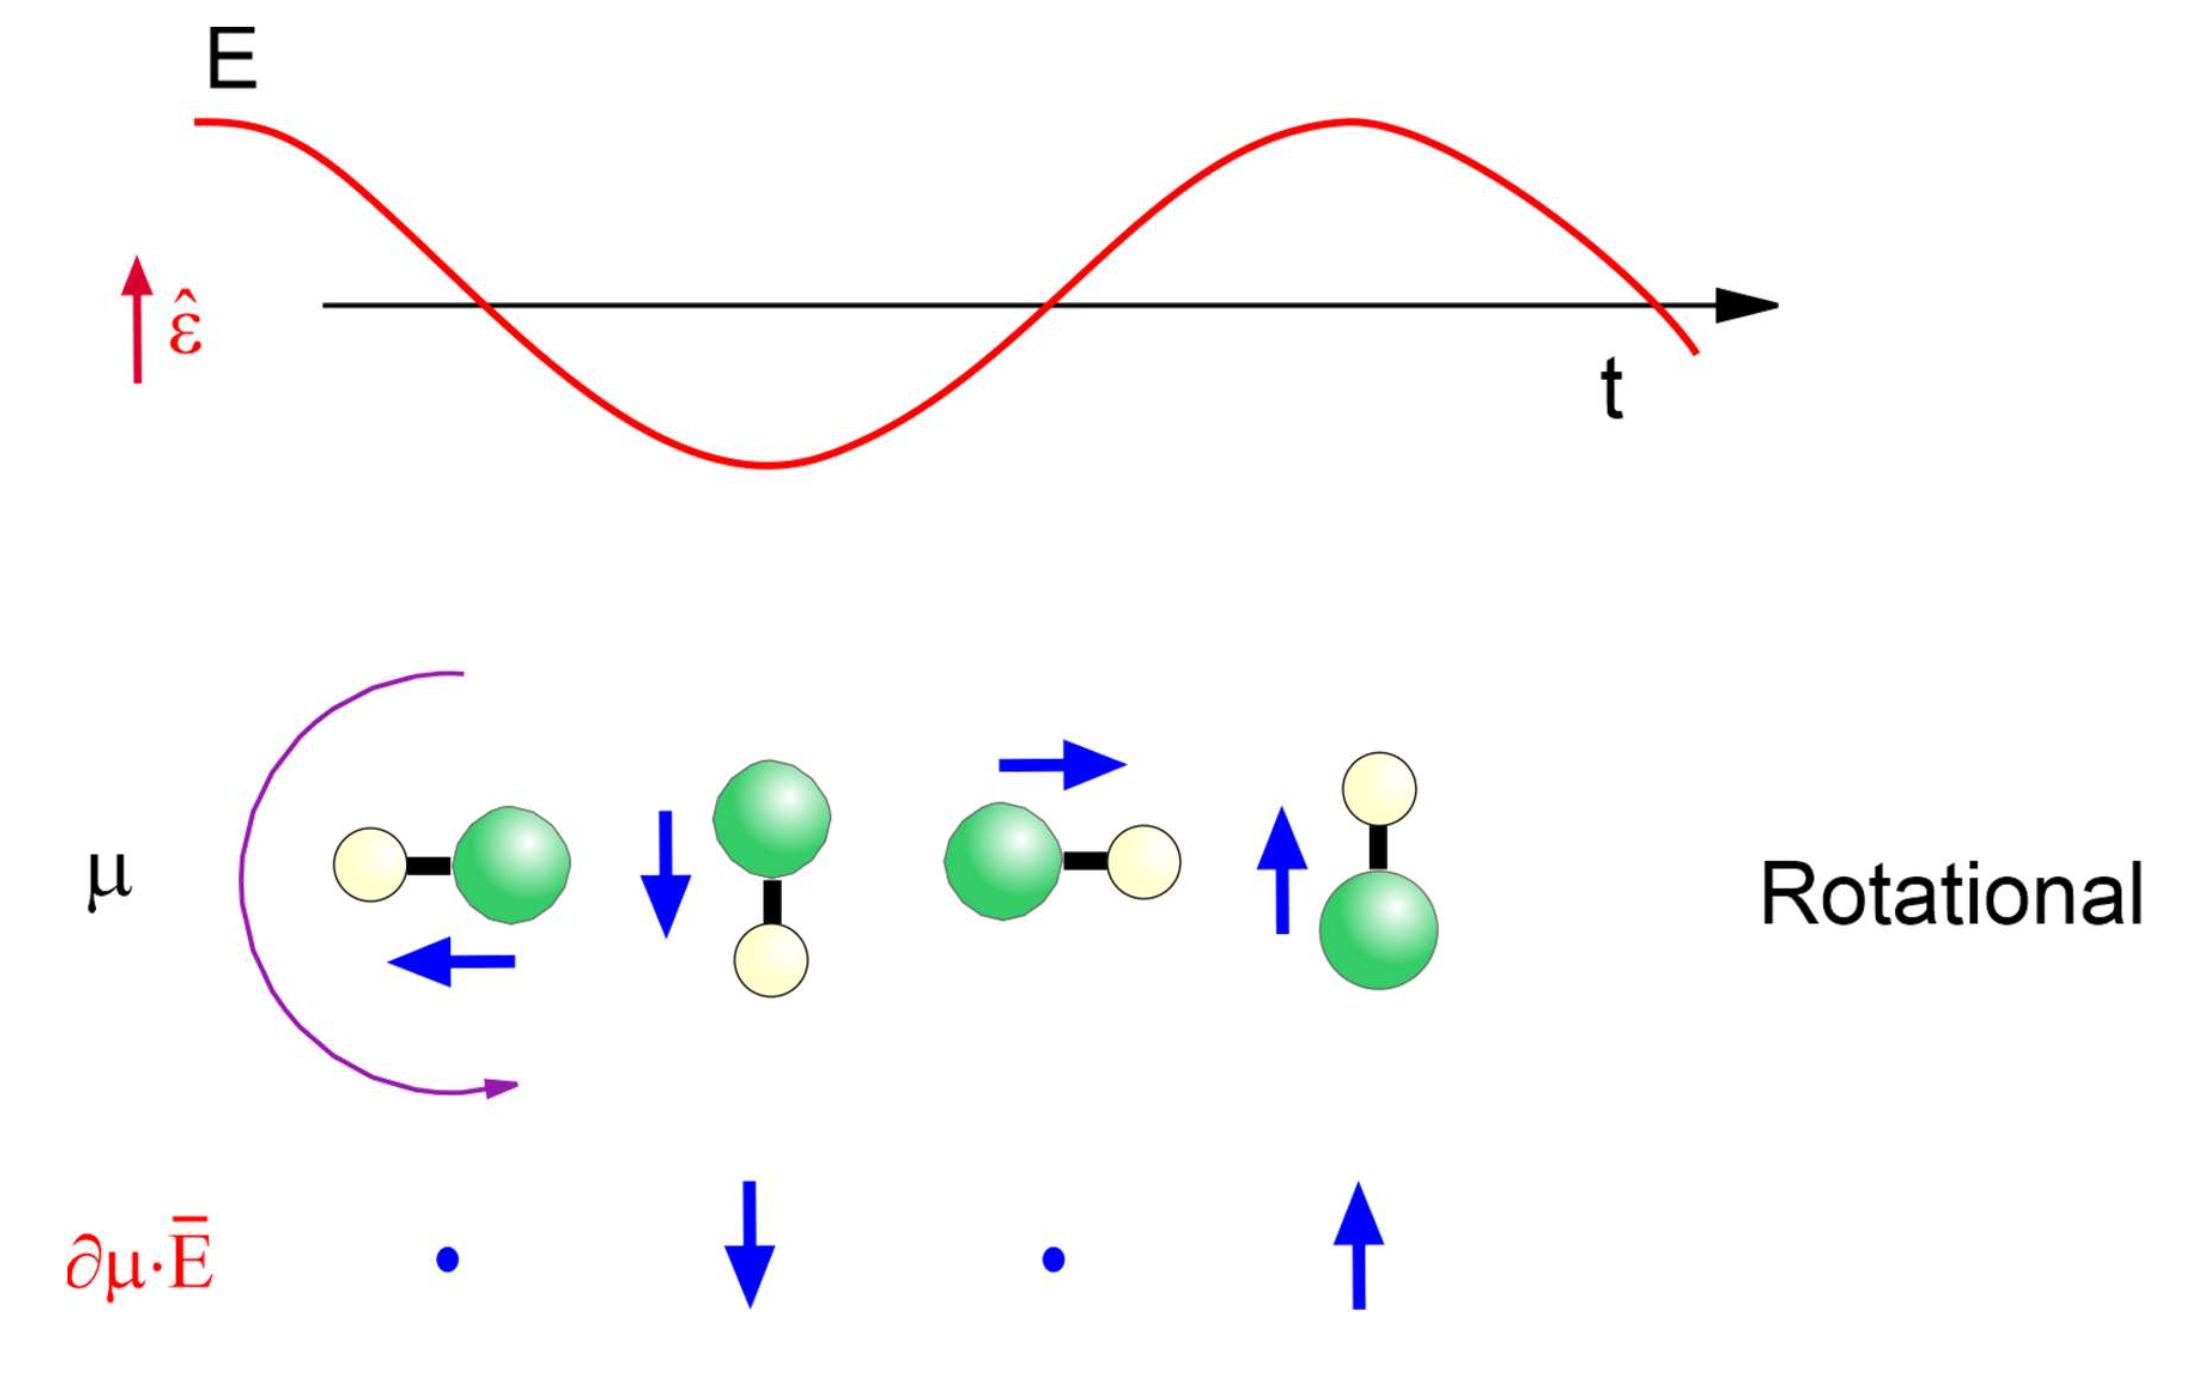
\includegraphics[width=0.47\linewidth]{EMrotationSync.png}
        \caption{Absorption through rotation of a dipole.}
        \label{fig:EMrotationSync}
    \end{figure}
    \begin{itemize}
        \item The rotational period has to align with the light period in order for the vibration to be driven.
        \item This is the origin of rotational spectroscopy.
    \end{itemize}
    \item Summary.
    \begin{itemize}
        \item We've developed a classical model for the interaction of a resonant field with charged particles.
        \item The observables in an absorption spectrum when classically described are the\dots
        \begin{itemize}
            \item Resonance frequency $\omega_0=\sqrt{k/m}$ where $\omega_0$ is both the natural periodic motion that displaces charges and the spectrum peak position, and $k$ is the quantum mechanical electronic structure holding the molecule together.
            \item Line width $\gamma$: Irreversible chemical relaxation processes and chemical rate processes.
            \item Peak amplitude: A proxy for the \textbf{extinction coefficient} $\varepsilon$.
            \begin{equation*}
                \frac{F_0^2}{2m\gamma} = \frac{I}{m\varepsilon_0\gamma}\left| \pdv{\bar{\mu}(\omega)}{Q} \right|^2\langle \cos^2\theta \rangle
            \end{equation*}
        \end{itemize}
    \end{itemize}
\end{itemize}




\end{document}